% \input{Functional}

\subsection{Functional Viewpoint}

\begin{itemize}
\item Related stakeholders: KLM, Initiator, EU-Claim
\item Related Concerns: Users of the system, Available functionality to each user group, Grouping functionalities
\item Related design decisions: EU-Claim can see private conversation after invitation, Online payment system (Discarded), Functionalities of Reporting System.
\end{itemize}

\newpage
\begin{landscape}
\begin{figure}
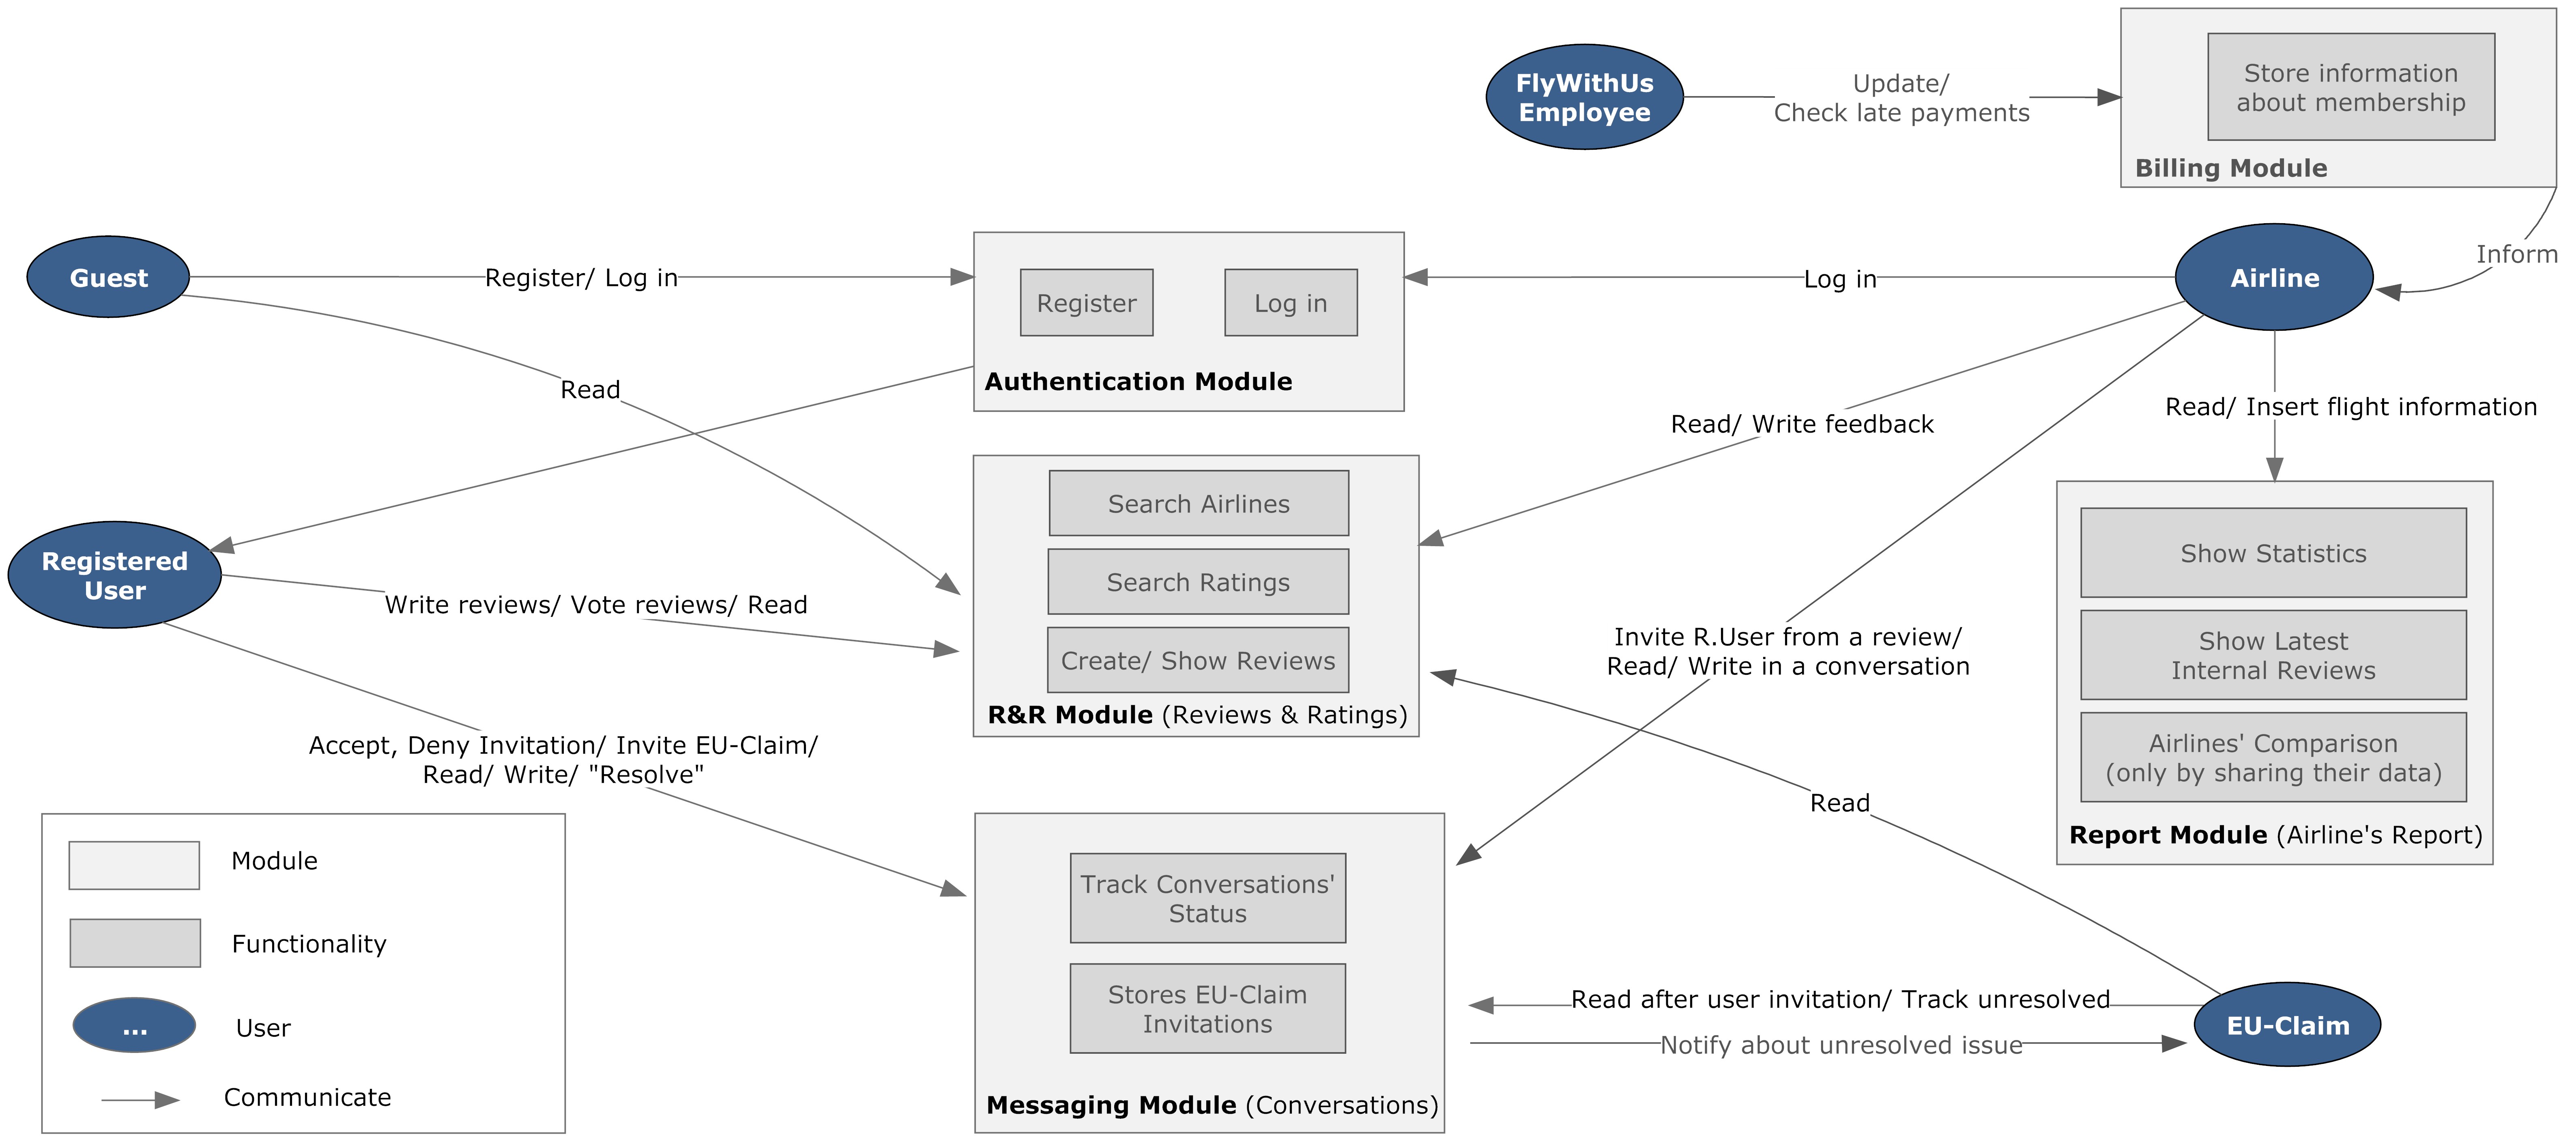
\includegraphics[width=600px]{Functional_Viewpoint.jpg}
\caption{Functional Viewpoint}
\label{fig:functional}
\end{figure}
\end{landscape}

The functional viewpoint (Fig.~\ref{fig:functional}) illustrates the users and the functionalities of the system. The functionalities
 that are based in the same entities of the system are grouped together to help the reader understand their connections. For example, all the functionalities 
 provided only to airlines are included in a {\em report} as a result these functionalities are grouped in the {\em Report System}. Furthermore, the viewpoint also presents the 
 availability of the functionalities to each user group and the communication between these groups through the system. For instance, a guest can register or log in the system and
 become a registered user, or an airline can invite a user to a private conversation in order to resolve a potential complaint; then the user can accept the invitation and he/ she can 
 also invite EU-Claim to monitor their conversation to ensure the integrity of this process.